Partiendo de la construcción de un vector ${\vec{\rho}}$ en ${r^{3}}$ se analizará su magnitud o norma que luego será utilizada para la transformación de coordenadas en el sistema rectangular al esférico. Dadas las componentes ${ \left( x,y,z \right )} = \vec{\rho}$ del vector, se producen los segmentos ${x,y,z}$ como se muestra en la segunda figura de la siguiente imagen:

\begin{figure}[H]
  \centering
  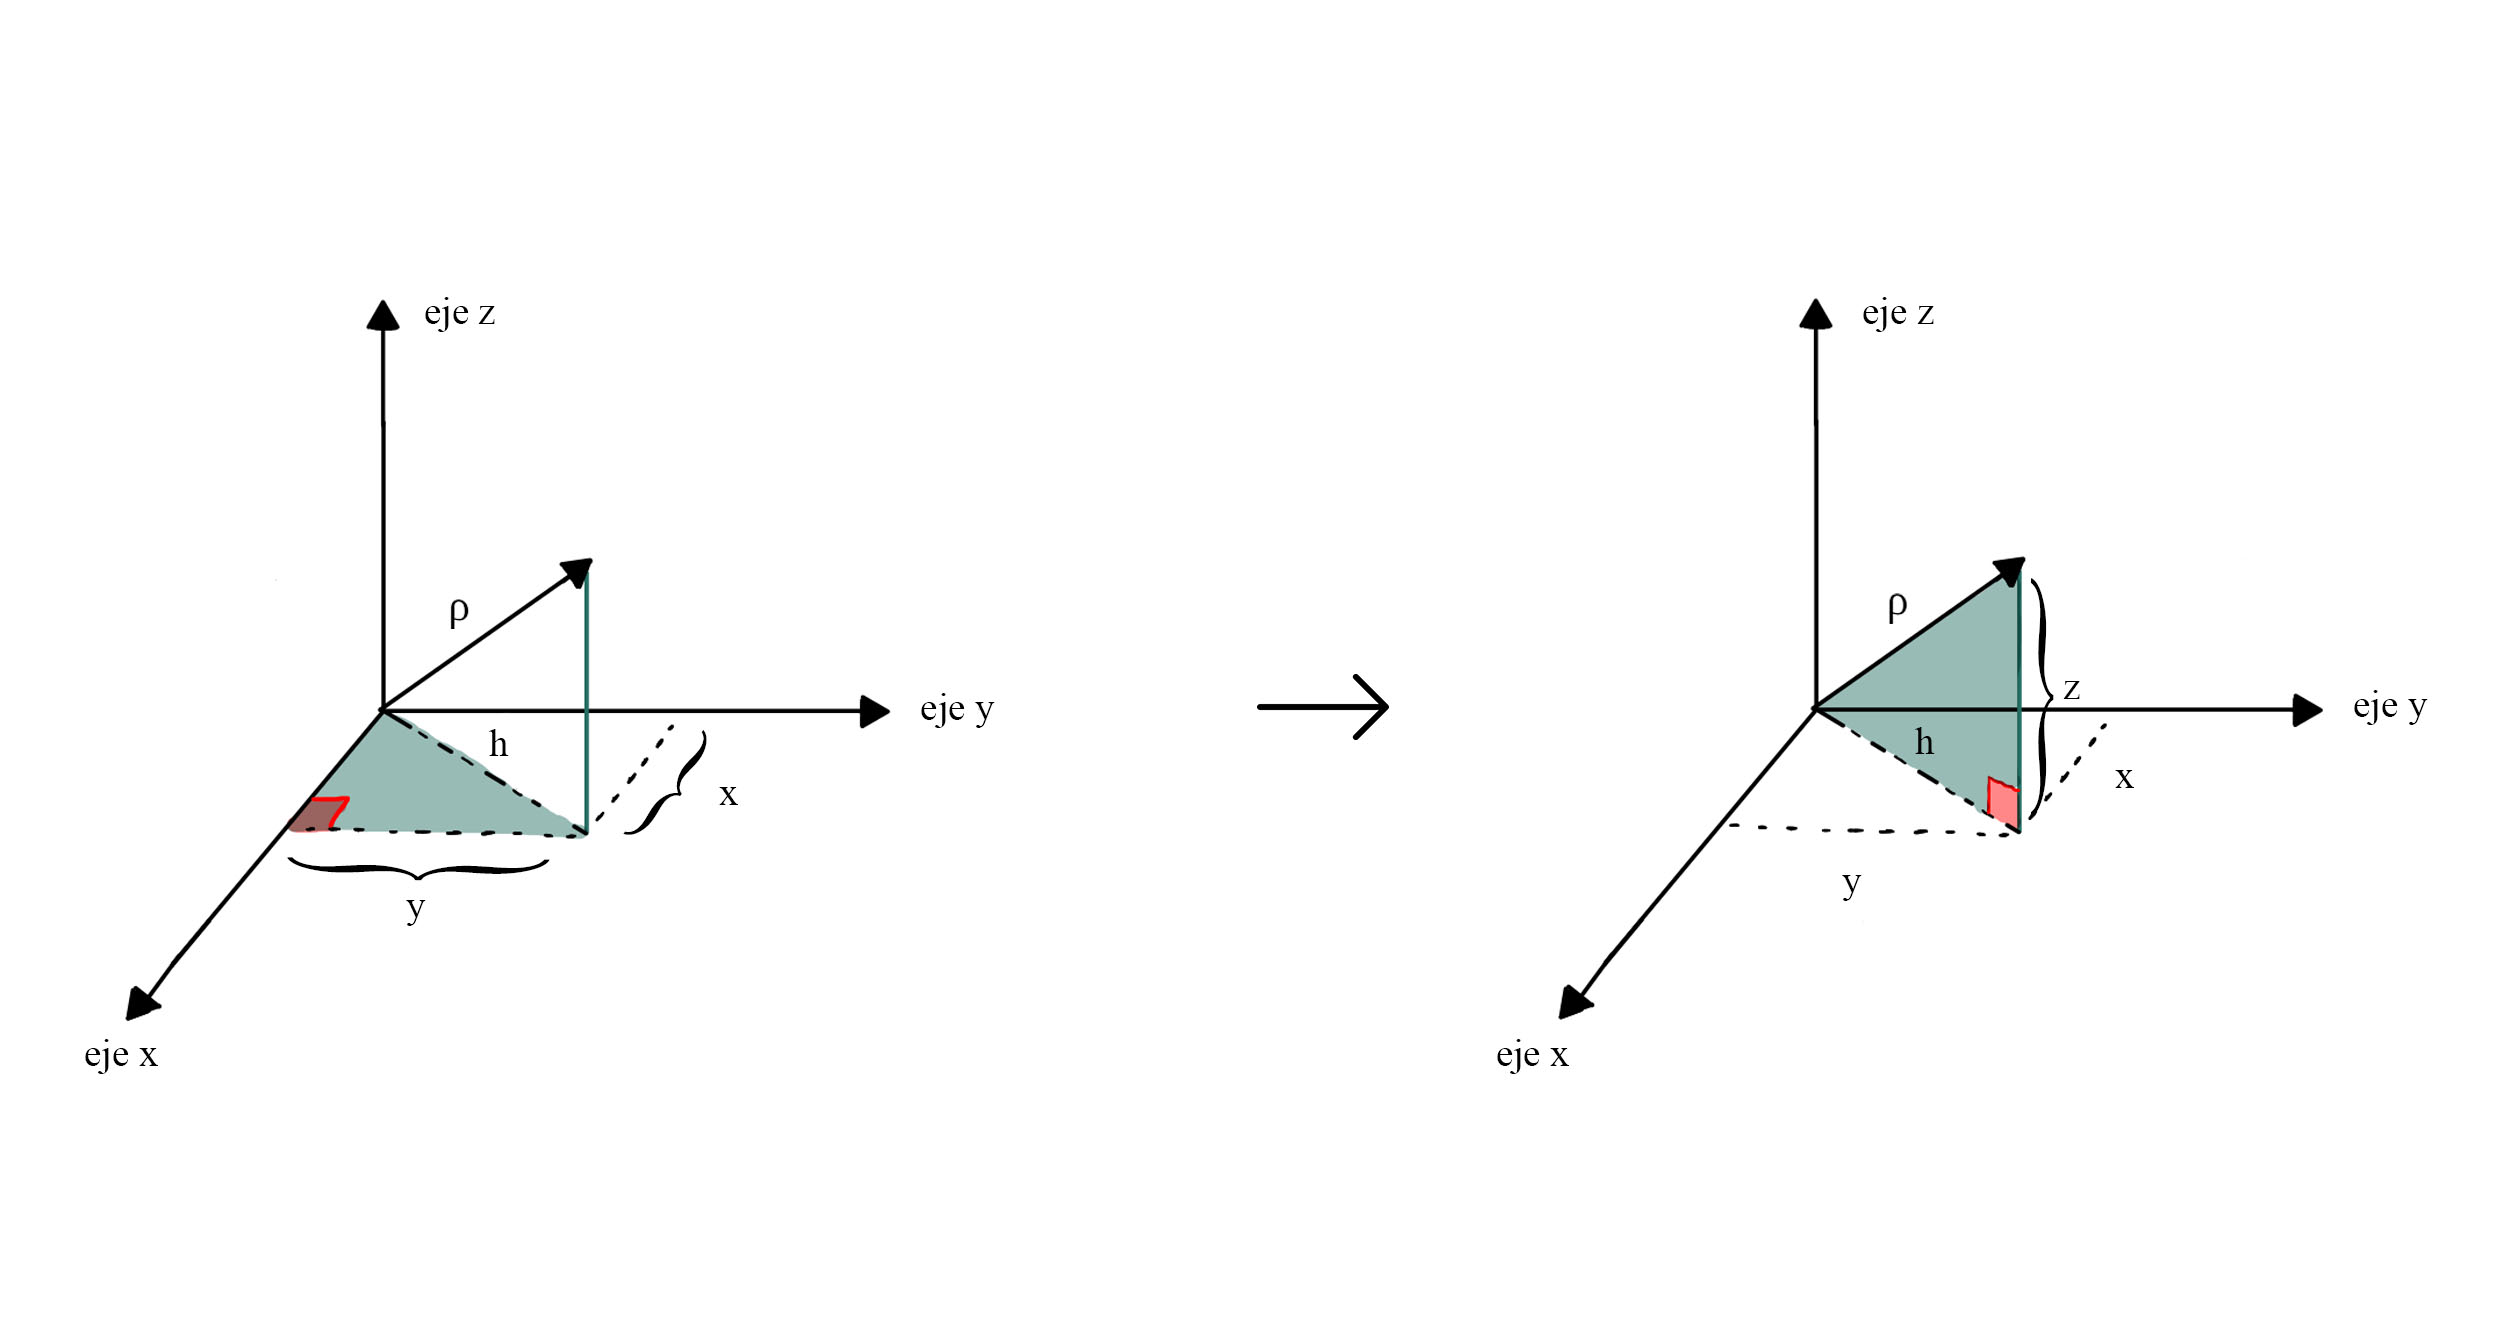
\includegraphics[width=11.17cm, height=5.67cm]{img/graph/norma_vectorial.jpg}
  \caption{Construcción de la norma de un vector ${\vec{\rho}}$.}
  \label{relacion_de_coordenadas}
\end{figure}

Ahora bien, analizando el triángulo rectángulo que se encuentra en el plano xy compuesto de hipotenusa ${h}$ y catetos ${x}$ y ${y}$, marcado de color verde en la primera figura, se puede calcular el valor de la hipotenusa utilizando el teorema de pitágoras.

\[ h = \sqrt{x^{2} + y^{2}} \]

\vspace{4mm}
De éste proceso se deriva el enfoque en el triángulo rectángulo formado por los catetos ${z}$ y ${h}$ e hipotenusa ${\rho}$, para el cual se calculará su valor.

\[ \rho = \sqrt{h^{2} + z^{2}} = \sqrt{\sqrt{x^{2} + y^{2}} + z^{2}} = \sqrt{x^{2} + y^{2} + z^{2} } \]

De acuerdo con la relación anterior se tiene el valor de una coordenada, ahora se desarrollará para los valores de los ángulos ${\theta}$ y ${\varphi}$. Recordando que ${z = \rho cos \varphi }$, entonces
\[cos\varphi = \frac{z}{\rho} \rightarrow cos^{-1} \left(\frac{z}{\rho}\right) = cos^{-1} \left(\frac{z}{\sqrt{x^{2} + y^{2} + z^{2} }}\right) = \varphi \]

Finalmente, considerando que en la tercera relación establecida en la introducción de la conversión de coordenadas, se sabe que ${\theta = tan^{-1}\left(\frac{y}{x}\right)}$, pero es importante señalar que en función del cuadrante será utilizada dicha relación. Así, se concluye que con las relaciones mencionadas podemos encontrar coordenadas en el sistema rectangular y convertirlo al sistema esférico.
